%\documentclass[notes,10pt,aspectratio=169]{beamer}

%\documentclass[notes, 10pt,aspectratio=169]{beamer}
\documentclass[10pt,aspectratio=169]{beamer}


% Add this line to your preamble
%\setbeameroption{show notes on second screen=right}

%\usetheme{Singapore} %Boadilla, Madrid, default, etc. 
\usetheme[progressbar=frametitle]{metropolis}
\usecolortheme{rose} %beaver, dolphin, crane, 


%\setbeamersize{text margin left=4mm, text margin right=4mm}


\usecolortheme{default}

\usepackage[utf8]{inputenc}
\usepackage[T1]{fontenc}
\usepackage{lmodern}
\usepackage{xcolor}
\usepackage{tikz}
\usepackage{booktabs} % Required for \toprule, \midrule, \bottomrule
\usetikzlibrary{shapes.geometric, arrows, positioning}

\tikzstyle{block} = [rectangle, draw, text width=4cm, align=center, rounded corners, minimum height=1cm]
\tikzstyle{decision} = [rectangle, draw, text width=5cm, align=center, fill=blue!10, rounded corners, minimum height=1cm]
\tikzstyle{terminal} = [rectangle, draw, text width=4.5cm, align=center, fill=yellow!30, rounded corners, minimum height=1cm]
\tikzstyle{end} = [rectangle, draw, text width=5cm, align=center, fill=green!30, rounded corners, minimum height=1cm]
\tikzstyle{arrow} = [->, thick]



\usepackage{adjustbox}
%2. change the bullets 
\setbeamertemplate{itemize item}[triangle] %circle, square,... 


% 1. Define custom colors and set colors 
%\definecolor{myblue}{HTML}{003366}
\definecolor{accent}{RGB}{78,205,196}

%\setbeamercolor{title}{fg=white,bg=myblue}
\setbeamercolor{frametitle}{fg=black,bg=white}
%\setbeamercolor{normal text}{fg=mygray}
\setbeamercolor{block title}{fg=black,bg=blue}
%\setbeamercolor{block body}{fg=black,bg=white}

\setbeamercolor{item}{fg= orange!80} % Change bullet color
\setbeamercolor{button}{bg=orange, fg=white}





% 3. BibLaTeX settings
\usepackage[
  backend=biber,
  style=apa,
  citestyle=authoryear
]{biblatex}
\addbibresource{references.bib}

\title{Equiilibrium effects of price updating: evidence from a centralized marketplace for annuities}
%\subtitle{A Mini Literature Overview}

\author{%
 Lucas Condeza
\inst{1} \and
   %\and
%  Coauthor Three\inst{3}
}
\institute{
  \inst{1} Yale University \\
}

\date{\today}

\begin{document}

\begin{frame}
  \titlepage
\end{frame}



 %%%%%%%%%

\begin{frame}{Motivation}
\begin{itemize}
    \item  Before beginning: in red aspects I especially would like to get feedback on. 
\end{itemize}
\end{frame}

%%%%%%%%%

\begin{frame}{This research}
\begin{itemize}
    \item 
\end{itemize}
\end{frame}

 %%%%%%%%%

\begin{frame}{Literature}
\begin{itemize}
    \item Aftermarkets: \textcite{larsen_efficiency_2021, allen_search_2019}

    \item Competition in selection markets: \textcite{mahoney_imperfect_2017, cuesta_price_2018, cosconati_competing_2025}

    \item Selection in multiple dimensions: \textcite{finkelstein_adverse_2004} and Finkelstein and McGarry (2006).  
\end{itemize}

\end{frame}

%%%%%%%%%



\begin{frame}{Outline}
\begin{itemize}
    \item a
\end{itemize}
\end{frame}


\begin{frame}{Setting: centralized annuities marketplace}\label{slide:setting}
       
    \begin{itemize}%[<+->]
    \item SCOMP steps: 
    \begin{enumerate}
        \item Request of balance statement 
        \item Request for offers: asks for certain type of contracts (e.g. annuity)
        \item Insurers post initial prices (e.g. \$20 per \$1 of flow) \hyperlink{slide:fig5}{\beamerbutton{Offer Certificate}}
        \item Retiree chooses one of the insurers or asks for revised prices

    \end{enumerate}

        \item Revised prices: bargaining and information disclosure
        

    \item Firms competition 1. financing cost 2. prediction algorithm 

    \item Profits of firm $j$: 
    \begin{align*}
    \pi_{ji}(F) = S_i-  \mathbb{E}^j_{T} \left[\sum_{t=1}^T\frac{F}{(1+r_j)^t}|x_i \right]
    \end{align*}
    % if it was only financing cost, it would be a monopoly
    \end{itemize}

     $S$: stock of savings, $F$: per period annuity payment, $x_i$: individual mortality factors
    
    \note{
    \begin{itemize}
        \item Explicitly not link the annuities market with pensions because generates confusion
        \item Explain what annuities are. 
    \end{itemize}}
\end{frame}


\begin{frame}{Data} \label{slide:data}
\begin{itemize}
    \item SCOMP data at the individual level  
    \begin{itemize}
        \item Posted and revised prices, and consumer decisions 
        \item Total savings 
        \item Demographics: age and gender \hyperlink{slide:fig5}{\beamerbutton{Certificate with initial prices}}
    \end{itemize}
     \item Retirement insurance companies: risk ratings
\end{itemize}
\note{Important to mention that the advantage of our data is that 1) elicits prices from almost all companies and 2) records all the elicited prices. }

\textcolor{red}{the particularity of our data is: }
\end{frame}

 

\begin{frame}{Descriptive Evidence}\label{slide:Descriptive_evidence}
\begin{itemize}
    \item Most buyers request external offers and the improvement is sizeable. \hyperlink{slide:fig1}{\beamerbutton{Search by income}} 
    \item Products are differentiated \hyperlink{slide:fig2}{\beamerbutton{Foregone value}} 
    \item Firms learn about other firms' prices
\end{itemize}
\end{frame}


%%%%%%%%%%%%%%%%%%%%%%%%%%%%%%%%%%%%%%%%%%%%%%%%%%%%%%

\begin{frame}\frametitle{Different use of the aftermarket}\label{slide:fig1}
\begin{figure}
    \centering
    \includegraphics[width=0.49\textwidth]{../figures/IE3_dist_external_offers.png}
    \hfill 
    \includegraphics[width=0.49\textwidth]{../figures/IE3_offer_improvement_histogram.png}
\end{figure}

\begin{itemize}
    \item   75\% of the purchases are through external offers. 
     \hyperlink{slide:Descriptive_evidence}{\beamerbutton{Go back}} 
    
    \textcolor{red}{[What are the determinants of search? Search direction?] }
\end{itemize}

\note{
That only some people use the aftermarket suggest: 
\begin{itemize}
    \item There are search costs 
    \item Firms could be discriminating based on the search likelihood. 
\end{itemize}
Any assessment of the welfare effects of the aftermarket has to consider that by banning it buyers will save in search costs, but will not be able to improve on the initial posted prices. 

In a model where search costs are not correlated with valuations, the aftermarket prices by the sellers are the same as the initial prices.
}
\end{frame}

%%%%%%%%%%%%%%%%%%%%%%%%%%%%%%%%%%%%%%%%%%%%%%%%%%%%%%

\begin{frame}{Heterogeneity in preferences}\label{slide:fig2}    
Buyers do not always buy highest annuity. Average foregone value is 1.57 monthly wages.
\begin{figure}[H]
%\caption{}
\centering{}%
\begin{tabular}{cc}
\includegraphics[scale=0.25]{../figures/IE3_foregone_hist.png}
\end{tabular}
\end{figure}
\hyperlink{slide:answer1}{\beamerbutton{Go back}}
\end{frame}


%%%%%%%%%%%%%%%%%%%%%%%%%%%


\begin{frame}{Heterogeneity in preferences}\label{slide:fig3}    
Buyers do not always buy highest annuity. Average foregone value is 1.57 monthly wages.
\begin{figure}[H]
%\caption{}
\centering{}%
\begin{tabular}{cc}
\includegraphics[scale=0.25]{../figures/IE6/IE6_survival_year_all.png}
\end{tabular}
\end{figure}
\hyperlink{slide:answer1}{\beamerbutton{Go back}}
\end{frame}


\begin{frame}%{Learning}
{
\def\sym#1{\ifmmode^{#1}\else\(^{#1}\)\fi}
\begin{tabular}{l*{7}{c}}
\hline\hline
                    &\multicolumn{1}{c}{(1)}&\multicolumn{1}{c}{(2)}&\multicolumn{1}{c}{(3)}&\multicolumn{1}{c}{(4)}&\multicolumn{1}{c}{(5)}&\multicolumn{1}{c}{(6)}&\multicolumn{1}{c}{(7)}\\
                    &\multicolumn{1}{c}{Increase}&\multicolumn{1}{c}{Increase}&\multicolumn{1}{c}{Increase}&\multicolumn{1}{c}{Increase}&\multicolumn{1}{c}{Increase}&\multicolumn{1}{c}{Increase}&\multicolumn{1}{c}{Has External Offer}\\
\hline
main                &                     &                     &                     &                     &                     &                     &                     \\
Avg. Gap            &       0.316\sym{***}&       0.155\sym{***}&       0.155\sym{***}&       0.139\sym{***}&       0.147\sym{***}&       0.071\sym{***}&                     \\
                    &     (0.006)         &     (0.010)         &     (0.010)         &     (0.016)         &     (0.019)         &     (0.020)         &                     \\
[1em]
Max. Gap            &                     &       0.110\sym{***}&       0.110\sym{***}&                     &      -0.021         &      -0.006         &                     \\
                    &                     &     (0.009)         &     (0.009)         &                     &     (0.029)         &     (0.028)         &                     \\
[1em]
gap\_from\_avg        &                     &                     &                     &                     &                     &                     &      -0.191\sym{***}\\
                    &                     &                     &                     &                     &                     &                     &     (0.032)         \\
[1em]
Constant            &       1.893\sym{***}&       1.375\sym{***}&       1.375\sym{***}&       1.381\sym{***}&       1.387\sym{***}&       1.511\sym{***}&      -2.012\sym{***}\\
                    &     (0.010)         &     (0.082)         &     (0.082)         &     (0.045)         &     (0.046)         &     (0.121)         &     (0.028)         \\
\hline
Observations        &       14133         &       14133         &       14133         &        2046         &        2046         &        2046         &       16164         \\
\hline\hline
\multicolumn{8}{l}{\footnotesize Average: is the difference between the mean of other firms' initial offers and own initial offer}\\
\multicolumn{8}{l}{\footnotesize Max Gap: is the difference between the highest other firm's initial offer and own initial offer.}\\
\multicolumn{8}{l}{\footnotesize Cols (1)-(3) use the population of initial offers that are not the highest, (4)-(6) only use the highest offer}\\
\multicolumn{8}{l}{\footnotesize Cols (4) and (6) include firm fixed effects}\\
\end{tabular}
}

\end{frame}

\begin{frame}{Learning(1)}
  \begin{figure}[H]
\caption{}
\label{fig:ie7_3}
\centering{}%
\begin{tabular}{cc}
\includegraphics[scale=0.39]{../figures/IE7/IE7_hist_bunching_max(2).png} 
\end{tabular}
\end{figure}
\end{frame}

\begin{frame}{}
\end{frame}

\begin{frame}{Initial prices}\label{slide:fig5}    
\begin{figure}[H]
%\caption{}
\centering{}%
\begin{tabular}{cc}
\includegraphics[scale=0.49]{../figures/annuity_offer.png}
\end{tabular}
\end{figure}
\hyperlink{slide:setting}{\beamerbutton{Go back}}
\end{frame}
%%%%%%%%%%%%%%%%%%%%%%%%%%%%%%%%%%%%%%%%%%%%%%
%%%%%%%%%%%%%%%%%%%%%%%%%%%%%%%%%%%%%%%%%%%%%%
%%%%%%%%%%%%%%%%%%%%%%%%%%%%%%%%%%%%%%%%%%%%%%
%%%%%%%%%%%%%%%%%%%%%%%%%%%%%%%%%%%%%%%%%%%%%%
%%%%%%%%%%%%%%%%%%%%%%%%%%%%%%%%%%%%%%%%%%%%%%
%%%%%%%%%%%%%%%%%%%%%%%%%%%%%%%%%%%%%%%%%%%%%%
%%%%%%%%%%%%%%%%%%%%%%%%%%%%%%%%%%%%%%%%%%%%%%
%%%%%%%%%%%%%%%%%%%%%%%%%%%%%%%%%%%%%%%%%%%%%%
%%%%%%%%%%%%%%%%%%%%%%%%%%%%%%%%%%%%%%%%%%%%%%
%%%%%%%%%%%%%%%%%%%%%%%%%%%%%%%%%%%%%%%%%%%%%%
 
%%%%%%%%%%%%%%%%%%%%%%%%%%%%%%%%%%%%%%
 
\begin{frame}{Answer the question}\label{slide:answer1}
    \begin{itemize}
        \item Equilibrium model of search and revised prices  
        \begin{itemize}
            \item First stage: sellers post initial prices and consumers buy or search 
            \item Second stage: If buyer searches is matched with a seller and they bargain
        \end{itemize}
        \item Desiderata:
        \begin{itemize}
           \item Imperfect-assymmetric competition\hyperlink{slide:fig2}{\beamerbutton{Evidence}}
            \item Differentiated products   \hyperlink{slide:fig3}{\beamerbutton{Evidence}}
            \item Adverse selection
        \end{itemize}
    \end{itemize}

    \textcolor{red}{[How to model selection with competition?]}
    \note{\textbf{ Imperfect-assymmetric competition:} the differences in market share can be due to preferences, but not so the differences in probability of posting a price
   
   \textbf{Diff products:} if not the case then everyone would choose the lowest price
   }
\end{frame}


    
% **CHANGES MARKED**: New slide added at end with simplified English SCOMP flow diagram

\begin{frame}{SCOMP Process Flow Diagram}
\begin{center}
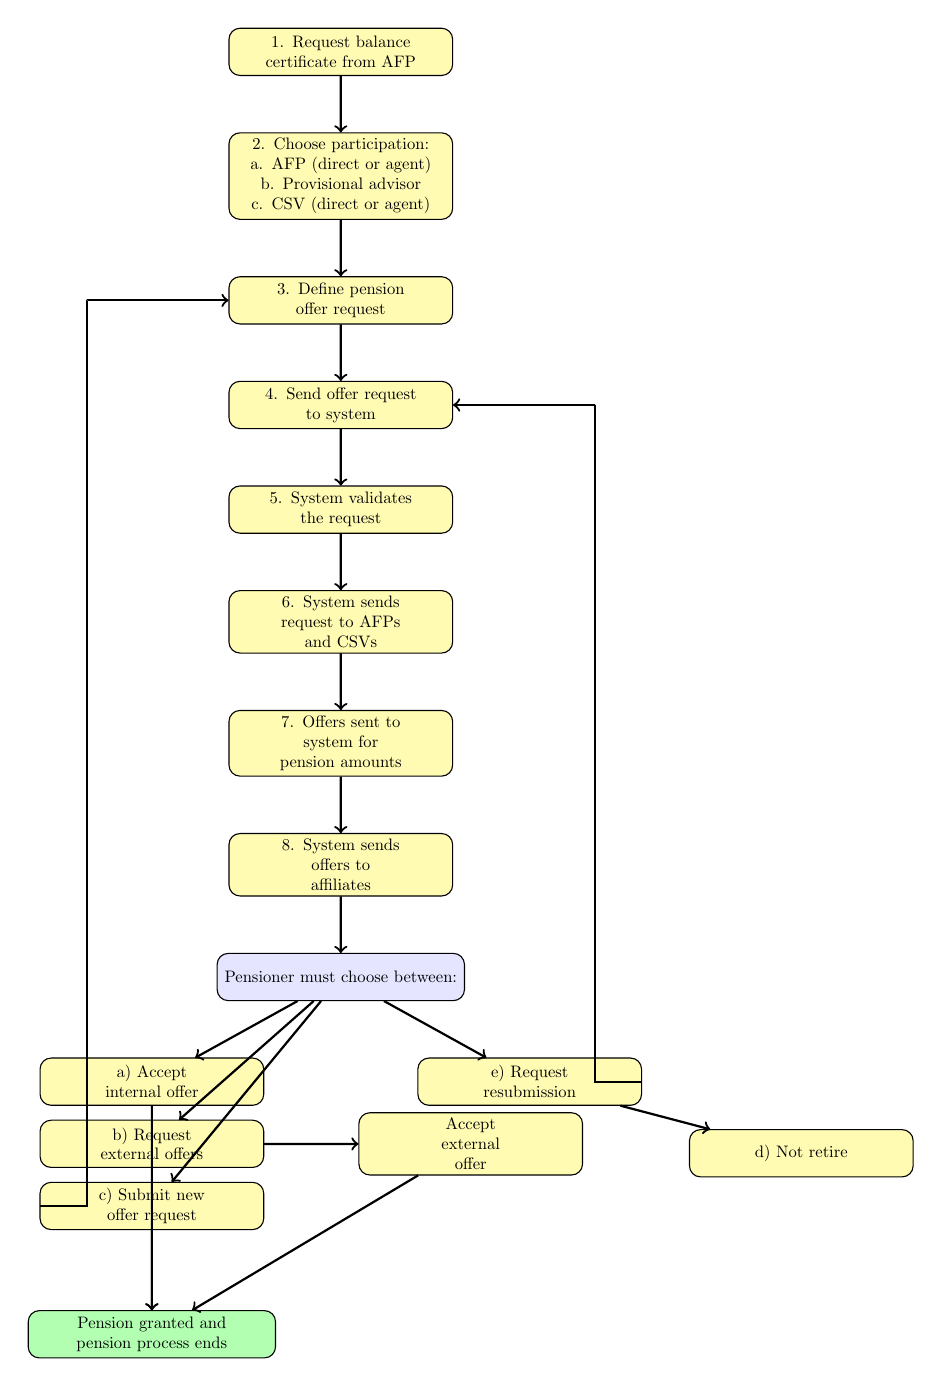
\begin{tikzpicture}[node distance=1.2cm, scale=0.6, every node/.style={transform shape}]

% **CHANGES MARKED**: Removed main process boxes (affiliate, participate, system, offers)
% **CHANGES MARKED**: Kept only numbered steps in sequential order

% Sequential numbered steps
\node[terminal] (step1) {1. Request balance\\certificate from AFP};
\node[terminal, below=of step1] (step2) {2. Choose participation:\\a. AFP (direct or agent)\\b. Provisional advisor\\c. CSV (direct or agent)};
\node[terminal, below=of step2] (step3) {3. Define pension\\offer request};
\node[terminal, below=of step3] (step4) {4. Send offer request\\to system};
\node[terminal, below=of step4] (step5) {5. System validates\\the request};
\node[terminal, below=of step5] (step6) {6. System sends\\request to AFPs\\and CSVs};
\node[terminal, below=of step6] (step7) {7. Offers sent to\\system for\\pension amounts};
\node[terminal, below=of step7] (step8) {8. System sends\\offers to\\affiliates};

% Decision node
\node[decision, below=of step8] (decision) {Pensioner must choose between:};

% Choice options
\node[terminal, below left=1.2cm and -1cm of decision] (choice_a) {a) Accept\\internal offer};
\node[terminal, below=0.3cm of choice_a] (choice_b) {b) Request\\external offers};
\node[terminal, below=0.3cm of choice_b] (choice_c) {c) Submit new\\offer request};
\node[terminal, below right=1.2cm and -1cm of decision] (choice_e) {e) Request\\resubmission};

% External offers path
\node[terminal, right=2cm of choice_b] (external) {Accept\\external\\offer};

% Final outcomes
\node[end, below=of choice_c, yshift=-0.5cm] (pension) {Pension granted and\\pension process ends};
\node[terminal, below right=0.5cm and 1cm of choice_e] (no_pension) {d) Not retire};

% **CHANGES MARKED**: Sequential arrows through numbered steps
\draw[arrow] (step1) -- (step2);
\draw[arrow] (step2) -- (step3);
\draw[arrow] (step3) -- (step4);
\draw[arrow] (step4) -- (step5);
\draw[arrow] (step5) -- (step6);
\draw[arrow] (step6) -- (step7);
\draw[arrow] (step7) -- (step8);
\draw[arrow] (step8) -- (decision);

% Decision paths
\draw[arrow] (decision) -- (choice_a);
\draw[arrow] (decision) -- (choice_b);
\draw[arrow] (decision) -- (choice_c);
\draw[arrow] (decision) -- (choice_e);

% External offer path
\draw[arrow] (choice_b) -- (external);
\draw[arrow] (external) -- (pension);

% Outcomes
\draw[arrow] (choice_a) -- (pension);
\draw[arrow] (choice_c) -- (pension);
\draw[arrow] (choice_e) -- (no_pension);

% Loop back arrows
\draw[arrow] (choice_c) -| ([xshift=-3cm]step3.west) |- (step3);
\draw[arrow] (choice_e) -| ([xshift=3cm]step4.east) |- (step4);

\end{tikzpicture}
\end{center}
\end{frame}


% **CHANGES MARKED**: New slide with horizontal left-to-right flow diagram in multiple rows

\begin{frame}{SCOMP Process Flow Diagram}
\begin{center}
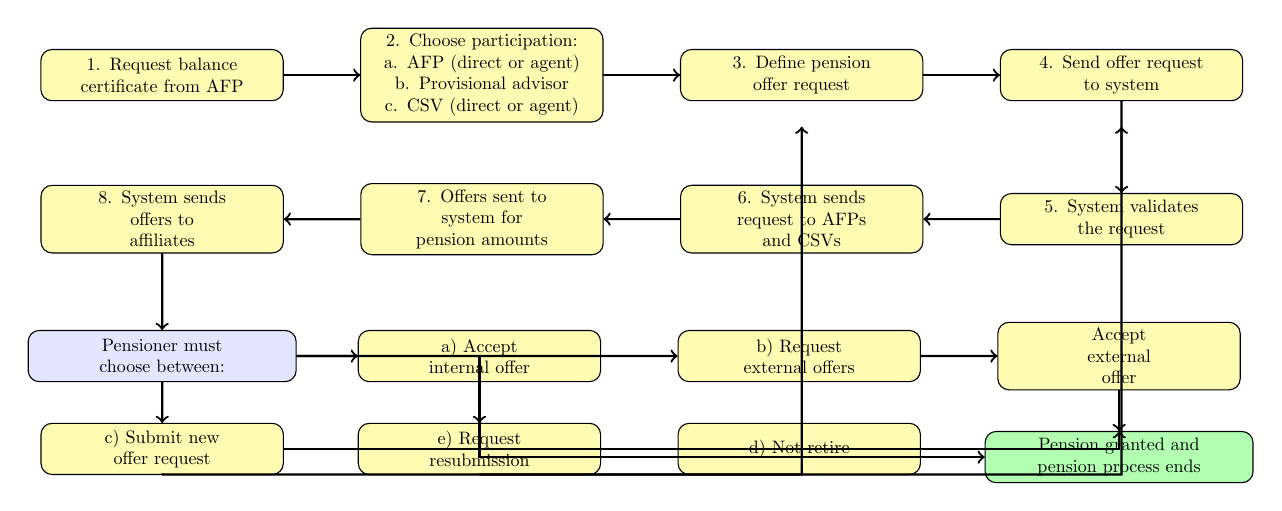
\begin{tikzpicture}[node distance=1.8cm and 1.5cm, scale=0.65, every node/.style={transform shape}]

% **CHANGES MARKED**: First row - left to right
\node[terminal] (step1) {1. Request balance\\certificate from AFP};
\node[terminal, right=of step1] (step2) {2. Choose participation:\\a. AFP (direct or agent)\\b. Provisional advisor\\c. CSV (direct or agent)};
\node[terminal, right=of step2] (step3) {3. Define pension\\offer request};
\node[terminal, right=of step3] (step4) {4. Send offer request\\to system};

% **CHANGES MARKED**: Second row - right to left
\node[terminal, below=of step4] (step5) {5. System validates\\the request};
\node[terminal, left=of step5] (step6) {6. System sends\\request to AFPs\\and CSVs};
\node[terminal, left=of step6] (step7) {7. Offers sent to\\system for\\pension amounts};
\node[terminal, left=of step7] (step8) {8. System sends\\offers to\\affiliates};

% **CHANGES MARKED**: Third row - decision and outcomes (left to right)
\node[decision, below=1.5cm of step8] (decision) {Pensioner must\\choose between:};
\node[terminal, right=1.2cm of decision] (choice_a) {a) Accept\\internal offer};
\node[terminal, right=of choice_a] (choice_b) {b) Request\\external offers};
\node[terminal, right=of choice_b] (external) {Accept\\external\\offer};

% Additional choices below decision
\node[terminal, below=0.8cm of decision] (choice_c) {c) Submit new\\offer request};
\node[terminal, below=0.8cm of choice_a] (choice_e) {e) Request\\resubmission};
\node[terminal, below=0.8cm of choice_b] (no_pension) {d) Not retire};

% Final outcome
\node[end, below=0.8cm of external] (pension) {Pension granted and\\pension process ends};

% **CHANGES MARKED**: Horizontal flow arrows - first row (left to right)
\draw[arrow] (step1) -- (step2);
\draw[arrow] (step2) -- (step3);
\draw[arrow] (step3) -- (step4);

% **CHANGES MARKED**: Connect first row to second row
\draw[arrow] (step4) -- (step5);

% **CHANGES MARKED**: Second row arrows (right to left)
\draw[arrow] (step5) -- (step6);
\draw[arrow] (step6) -- (step7);
\draw[arrow] (step7) -- (step8);

% **CHANGES MARKED**: Connect second row to decision
\draw[arrow] (step8) -- (decision);

% Decision paths
\draw[arrow] (decision) -- (choice_a);
\draw[arrow] (decision) -- (choice_b);
\draw[arrow] (decision) -- (choice_c);
\draw[arrow] (decision) -| (choice_e);

% External offer path
\draw[arrow] (choice_b) -- (external);

% Outcomes to pension
\draw[arrow] (choice_a) |- (pension);
\draw[arrow] (external) -- (pension);
\draw[arrow] (choice_c) -| (pension);

% Loop back arrows
\draw[arrow] (choice_c) -- ++(0,-0.5) -| ([yshift=-0.5cm]step3.south);
\draw[arrow] (choice_e) -- ++(0,-0.5) -| ([yshift=-0.5cm]step4.south);

\end{tikzpicture}
\end{center}
\end{frame}


% **CHANGES MARKED**: Merged steps 3-4, and steps 5-6-7 into simplified flow

\begin{frame}{SCOMP Process Flow Diagram}
\begin{center}
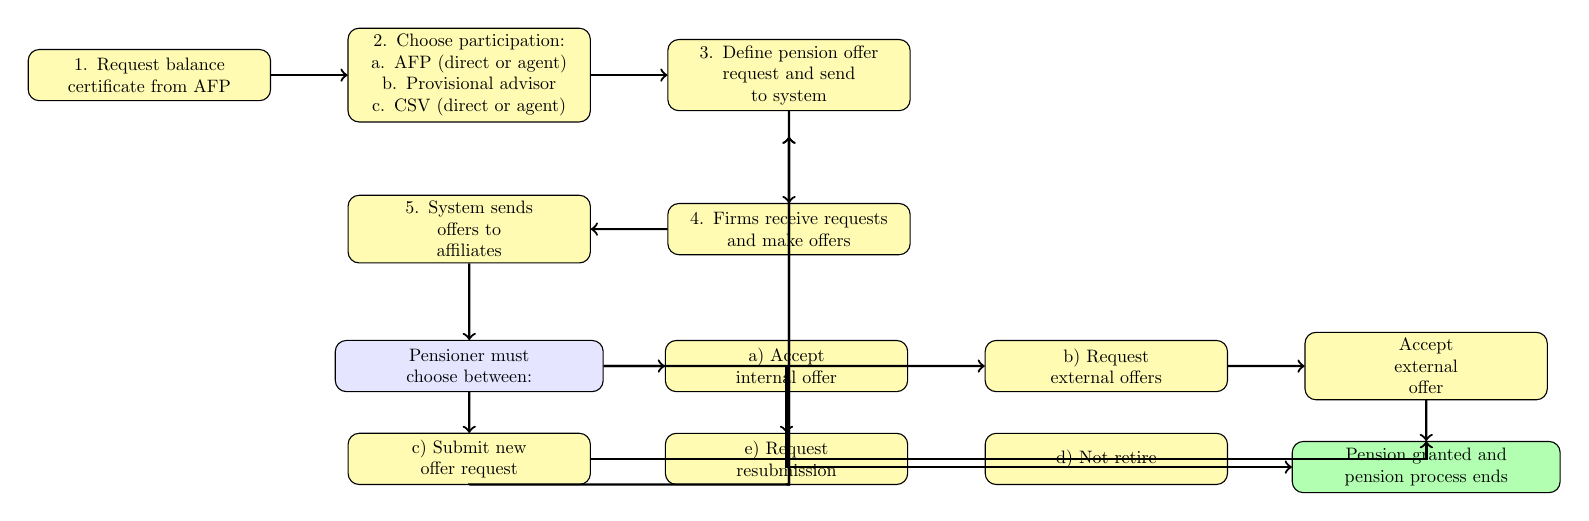
\begin{tikzpicture}[node distance=1.8cm and 1.5cm, scale=0.65, every node/.style={transform shape}]

% **CHANGES MARKED**: First row - left to right (3 steps now)
\node[terminal] (step1) {1. Request balance\\certificate from AFP};
\node[terminal, right=of step1] (step2) {2. Choose participation:\\a. AFP (direct or agent)\\b. Provisional advisor\\c. CSV (direct or agent)};
% **CHANGES MARKED**: Merged steps 3 and 4
\node[terminal, right=of step2] (step3) {3. Define pension offer\\request and send\\to system};

% **CHANGES MARKED**: Second row - right to left (2 steps now)
% **CHANGES MARKED**: Merged steps 5, 6, and 7
\node[terminal, below=of step3] (step4) {4. Firms receive requests\\and make offers};
\node[terminal, left=of step4] (step5) {5. System sends\\offers to\\affiliates};

% **CHANGES MARKED**: Third row - decision and outcomes (left to right)
\node[decision, below=1.5cm of step5] (decision) {Pensioner must\\choose between:};
\node[terminal, right=1.2cm of decision] (choice_a) {a) Accept\\internal offer};
\node[terminal, right=of choice_a] (choice_b) {b) Request\\external offers};
\node[terminal, right=of choice_b] (external) {Accept\\external\\offer};

% Additional choices below decision
\node[terminal, below=0.8cm of decision] (choice_c) {c) Submit new\\offer request};
\node[terminal, below=0.8cm of choice_a] (choice_e) {e) Request\\resubmission};
\node[terminal, below=0.8cm of choice_b] (no_pension) {d) Not retire};

% Final outcome
\node[end, below=0.8cm of external] (pension) {Pension granted and\\pension process ends};

% **CHANGES MARKED**: Horizontal flow arrows - first row (left to right, now 3 steps)
\draw[arrow] (step1) -- (step2);
\draw[arrow] (step2) -- (step3);

% **CHANGES MARKED**: Connect first row to second row
\draw[arrow] (step3) -- (step4);

% **CHANGES MARKED**: Second row arrows (right to left, now 2 steps)
\draw[arrow] (step4) -- (step5);

% **CHANGES MARKED**: Connect second row to decision
\draw[arrow] (step5) -- (decision);

% Decision paths
\draw[arrow] (decision) -- (choice_a);
\draw[arrow] (decision) -- (choice_b);
\draw[arrow] (decision) -- (choice_c);
\draw[arrow] (decision) -| (choice_e);

% External offer path
\draw[arrow] (choice_b) -- (external);

% Outcomes to pension
\draw[arrow] (choice_a) |- (pension);
\draw[arrow] (external) -- (pension);
\draw[arrow] (choice_c) -| (pension);

% **CHANGES MARKED**: Loop back arrows now go to merged step 3
\draw[arrow] (choice_c) -- ++(0,-0.5) -| ([yshift=-0.5cm]step3.south);
\draw[arrow] (choice_e) -- ++(0,-0.5) -| ([yshift=-0.5cm]step3.south);

\end{tikzpicture}
\end{center}
\end{frame}



\begin{frame}{SCOMP Process Flow Diagram}
\begin{center}
\begin{tikzpicture}[node distance=1.8cm and 1.5cm, scale=0.6, every node/.style={transform shape}]

% **CHANGES MARKED**: First row - left to right
\node[terminal] (step1) {1. Request balance\\certificate from AFP};
\node[terminal, right=of step1] (step2) {2. Choose participation:\\a. AFP (direct or agent)\\b. Provisional advisor\\c. CSV (direct or agent)};
\node[terminal, right=of step2] (step3) {3. Define offer request \\ and send it to the system};
\node[terminal, right=of step3] (step4) {4. System sends\\request to AFPs\\and CSVs, who \\ make their offers};

% **CHANGES MARKED**: Second row - right to left
%\node[terminal, below=of step4] (step5) {5. Offers sent to\\system for\\pension amounts};
\node[terminal, below =of step4] (step6) {5. System sends\\offers to\\affiliates};
\node[decision, left=of step6] (step7) {6. Pensioner must\\choose between:};


% **CHANGES MARKED**: Third row - decision and outcomes (left to right)
%\node[decision, below=1.5cm of step8] (decision) {Pensioner must\\choose between:};
\node[terminal, below=1.2cm of step7] (choice_b) {b) Request\\external offers};
\node[terminal, left=of choice_b] (choice_a) {a) Accept\\internal offer};
\node[terminal, right= of choice_b ] (choice_c) {c) Submit new\\offer request};
%\node[terminal, right=of choice_b] (external) {Accept\\external\\offer};

% Additional choices below decision

\node[terminal, below=0.8cm of choice_b] (no_pension) {d) Not retire};

% Final outcome
\node[end, below=0.8cm of external] (pension) {Pension granted and\\pension process ends};

% **CHANGES MARKED**: Horizontal flow arrows - first row (left to right)
\draw[arrow] (step1) -- (step2);
\draw[arrow] (step2) -- (step3);
\draw[arrow] (step3) -- (step4);

% **CHANGES MARKED**: Connect first row to second row
\draw[arrow] (step4) -- (step5);

% **CHANGES MARKED**: Second row arrows (right to left)
\draw[arrow] (step5) -- (step6);
\draw[arrow] (step6) -- (step7);
\draw[arrow] (step7) -- (choice_a);
\draw[arrow] (step7) -- (choice_b);
\draw[arrow] (step7) -- (choice_c);

% **CHANGES MARKED**: Connect second row to decision
%\draw[arrow] (step8) -- (decision);

% Decision paths
%\draw[arrow] (decision) -- (choice_a);
%\draw[arrow] (decision) -- (choice_b);
%\draw[arrow] (decision) -- (choice_c);
%\draw[arrow] (decision) -| (choice_e);

% External offer path
%\draw[arrow] (choice_b) -- (external);

% Outcomes to pension
%\draw[arrow] (choice_a) |- (pension);
%\draw[arrow] (external) -- (pension);
%\draw[arrow] (choice_c) -| (pension);

% Loop back arrows
%\draw[arrow] (choice_c) -- ++(0,-0.5) -| ([yshift=-0.5cm]step3.south);
%\draw[arrow] (choice_e) -- ++(0,-0.5) -| ([yshift=-0.5cm]step4.south);

\end{tikzpicture}
\end{center}
\end{frame}

\end{document}